\lab{Conditioning and Stability}{Conditioning and Stability}
\objective{The condition number of a function measures how sensitive that function is to changes in the input.
On the other hand, the stability of an algorithm measures how accurately that algorithm computes the value of a function from exact input.
Both of these concepts are important for answering the crucial question, ``is my computer telling the truth?''
In this lab, we examine the conditioning of common linear algebra problems, including computing polynomial roots and matrix eigenvalues.
We also present an example to demonstrate how two different algorithms for the same problem may not have the same level of stability.}

\section*{Conditioning} % =====================================================

The \emph{absolute condition number} of a function $f: \mathbb{R}^m \rightarrow \mathbb{R}^n$ at a point $\x\in\mathbb{R}^m$ is defined by
\begin{equation}
\hat{\kappa} (\x) = \lim_{\delta \rightarrow 0^+} \sup_{\norm{\mathbf{h}} < \delta} { \frac{\norm{f(\x + \mathbf{h} ) - f(\x)}}{\norm{\mathbf{h}}} }.
\label{eq:absolute-condition-number}
\end{equation}

In other words, the absolute condition number of $f$ is the limit of the change in output over the change of input.
Similarly, the \emph{relative condition number} of $f$ is the limit of the relative change in output over the relative change in input,
\begin{equation}
\kappa(\x)
= \lim_{\delta \rightarrow 0^+} \sup_{\norm{\mathbf{h}} < \delta} \left({ \frac{\norm{f(\x + \mathbf{h} ) - f(\x)}}{\norm{f(\x)}} } \middle/ { \frac{\norm{\mathbf{h}}}{\norm{\x}} }\right)
= \frac{\norm{\x}}{\norm{f(\x)}} \hat{\kappa}(\x).
\label{eq:relative-condition-number}
\end{equation}

A function with a large condition number is called \emph{ill-conditioned}.
Small changes to the input of an ill-conditioned function may produce large changes in output.
It is important to know if a function is ill-conditioned because floating point representation almost always introduces some input error, and therefore the outputs of ill-conditioned functions cannot be trusted.

The \emph{condition number} of a matrix $A$, $\kappa (A)=\|A\| \|A^{-1}\|$, is an upper bound on the condition number for many of the common problems associated with the matrix, such as solving the system $A\x =\b$.
If $A$ is square but not invertible, then $\kappa(A) = \infty$ by convention.
To compute $\kappa(A)$, we often use the matrix 2-norm, which is the largest singular value $\sigma_{\max}$ of $A$.
Recall that if $\sigma$ is a singular value of $A$, $\frac{1}{\sigma}$ is a singular value of $A^{-1}$.
Thus, we have that
\begin{equation}\label{eq:matrix_cond}
\kappa(A) = \frac{\sigma_{\max}}{\sigma_{\min}},
\end{equation}
which is also a valid equation for non-square matrices.

\begin{warn} % Ill-conditioned matrices.
Ill-conditioned matrices can wreak havoc in even simple applications.
% Solving problems can become difficult or even impossible when working with matrices that have large condition numbers because small changes in input can quickly lead to inaccurate output.
For example, the matrix
\[
A =
\left[\begin{array}{cc}
1 & 1 \\
1 & 1.0000000001
\end{array}\right]
\]
is extremely ill-conditioned, with $\kappa(A) \approx 4\times 10^{10}$.
Solving the systems $A\x = \b_1$ and $A\x = \b_2$ can result in wildly different answers, even when $\b_1$ and $\b_2$ are extremely close.

\begin{lstlisting}
>>> import numpy as np
>>> from scipy import linalg as la

>>> A = np.array([[1, 1], [1, 1+1e-10]])
>>> np.linalg.cond(A)
39999991794.058899

# Set up and solve a simple system of equations.
>>> b1 = np.array([2, 2])
>>> x1 = la.solve(A, b1)
>>> print(x1)
[ 2.  0.]

# Solve a system with a very slightly different vector b.
>>> b2 = np.array([2, 2+1e-5])
>>> la.norm(b1 - b2)
>>> x2 = la.solve(A, b2)
>>> print(x2)
[-99997.99172662  99999.99172662]   # This solution is hugely different!
\end{lstlisting}

If you find yourself working with matrices that have large condition numbers, check your math carefully or try to reformulate the problem entirely.
\end{warn}

\begin{info} % Orthonormal matrices are the best!
An \emph{orthonormal matrix} $U$ has orthonormal columns and satisfies $U\trp U = I$ and $\|U\|_2 = 1$.
If $U$ is square, then $U^{-1} = U\trp$ and $U\trp$ is also orthonormal.
Therefore $\kappa(U) = \|U\|_2\|U^{-1}\|_2 = 1$.
Even if $U$ is not square, all of its singular values are equal to $1$, and again $\kappa(U) = \sigma_{\max} / \sigma_{\min} = 1$.

The condition number of a matrix cannot be less than $1$ since $\sigma_{\max} \ge \sigma_{\min}$ by definition.
Thus orthonormal matrices are, in a sense, the best kind of matrices for computations.
This is one of the main reasons why numerical algorithms based on the QR decomposition or the SVD are so important.
\end{info}

\begin{problem} % Compute matrix condition number.
Write a function that accepts a matrix $A$ and computes its condition number using (\ref{eq:matrix_cond}).
Use \li{scipy.linalg.svd()}, or \li{scipy.linalg.svdvals()} to compute the singular values of $A$.
Avoid computing $A^{-1}$.
If the smallest singular value is $0$, return $\infty$ (\li{np.inf}).

Validate your function by comparing it to \li{np.linalg.cond()}.
Check that orthonormal matrices have a condition number of $1$ (use \li{scipy.linalg.qr()} to generate an orthonormal matrix) and that singular matrices have a condition number of $\infty$ according to your function.
\end{problem}

% For large matrices where taking the SVD is difficult, the exact condition number of a matrix cannot always be computed and therefore must be estimated.
% Although not covered here, there exist many algorithms that can efficiently and accurately estimate the condition number of a matrix.

\subsection*{The Wilkinson Polynomial} % --------------------------------------

Let $f:\mathbb{C}^{n+1} \rightarrow \mathbb{C}^n$ be the function that maps a collection of $n+1$ coefficients $(c_n, c_{n-1}, \ldots, c_0)$ to the $n$ roots of the polynomial $c_nx^n+c_{n-1}x^{n-1}+\ldots+c_2x^2+c_1x+c_0$.
Finding polynomial roots is an extremely ill-conditioned problem in general, so the condition number of $f$ is likely very large.
To see this, consider the \emph{Wilkinson polynomial}, made famous by James H. Wilkinson in 1963:
\[
w(x) = \prod_{r=1}^{20}(x-r) = x^{20} - 210x^{19} + 20615x^{18} - 1256850x^{17} + \cdots.
\]
Let $\tilde{w}(x)$ be $w(x)$ where the coefficient on $x^{19}$ is very slightly perturbed from $-210$ to $-210.0000001$.
The following code computes and compares the roots of $\tilde{w}(x)$ and $w(x)$ using NumPy and SymPy.

\begin{comment}
\begin{lstlisting}
>>> w_coeffs = np.array([1, -210, 20615, -1256850, 53327946, -1672280820,
                    40171771630, -756111184500, 11310276995381,
                    -135585182899530, 1307535010540395,
                    -10142299865511450, 63030812099294896,
                    -311333643161390640, 1206647803780373360,
                    -3599979517947607200, 8037811822645051776,
                    -12870931245150988800, 13803759753640704000,
                    -8752948036761600000, 2432902008176640000])
>>> w_roots = np.arange(1, 21)
\end{lstlisting}
\end{comment}

\begin{lstlisting}
>>> import sympy as sy
>>> from matplotlib import pyplot as plt

# The roots of w are 1, 2, ..., 20.
>>> w_roots = np.arange(1, 21)

# Get the exact Wilkinson polynomial coefficients using SymPy.
>>> x, i = sy.symbols('x i')
>>> w = sy.poly_from_expr(sy.product(x-i, (i, 1, 20)))[0]
>>> w_coeffs = np.array(w.all_coeffs())
>>> print(w_coeffs[:6])
[1 -210 20615 -1256850 53327946 -1672280820]

# Perturb one of the coefficients very slightly.
>>> h = np.zeros(21)
>>> h[1]=1e-7
>>> new_coeffs = w_coeffs - h
>>> print(new_coeffs[:6])
[1 -210.000000100000 20615 -1256850 53327946 -1672280820]

# Use NumPy to compute the roots of the perturbed polynomial.
>>> new_roots = np.roots(np.poly1d(new_coeffs))
\end{lstlisting}

Figure \ref{fig:wilkinson-perturbed-poly} plots $w(x)$ and $\tilde{w}(x)$ together, and Figure \ref{fig:wilkinon-perturbed-roots} and compares their roots in the complex plane.

\begin{figure}[H] % Original and pertubed Wilkinson polynomial + roots
\captionsetup[subfigure]{justification=justified}
\centering
\begin{subfigure}{.48\textwidth}
    \centering
    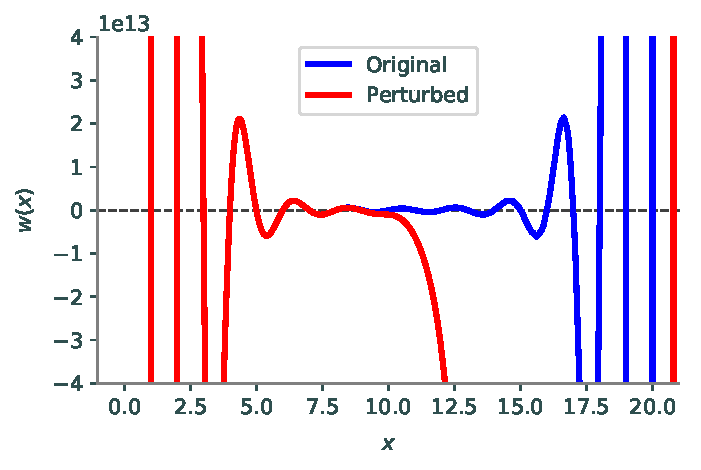
\includegraphics[width=\linewidth]{figures/perturbed_poly.pdf}
    \caption{The original and perturbed Wilkinson polynomials.
    They match for about half of the domain, then differ drastically.}
    \label{fig:wilkinson-perturbed-poly}
\end{subfigure}
\quad
\begin{subfigure}{.48\textwidth}
    \centering
    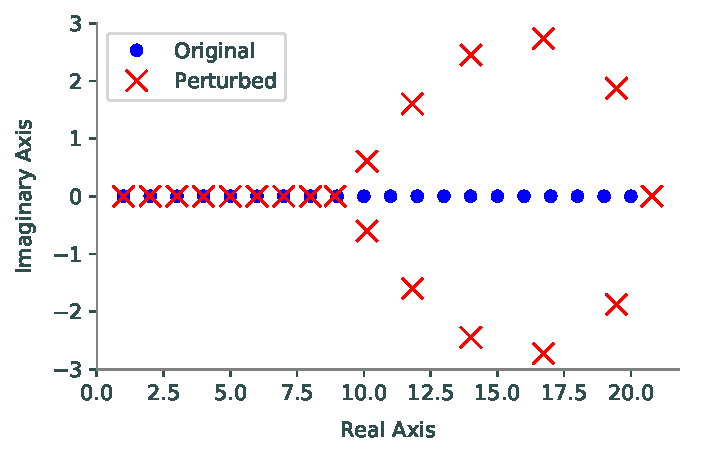
\includegraphics[width=\linewidth]{figures/perturbed_roots.pdf}
    \caption{Roots of the original and perturbed Wilkinson polynomials.
    About half of the perturbed roots are complex.}
    \label{fig:wilkinon-perturbed-roots}
\end{subfigure}
\caption{}
\label{fig:wilkinson-polynomial}
\end{figure}

Figure \ref{fig:wilkinson-polynomial} clearly indicates that a very small change in just a single coefficient drastically changes the nature of the polynomial and its roots.
To quantify the difference, estimate the condition numbers (this example uses the $\infty$ norm to compute $\hat{\kappa}$ and $\kappa$).

\begin{lstlisting}
# Sort the roots to ensure that they are in the same order.
>>> w_roots = np.sort(w_roots)
>>> new_roots = np.sort(new_roots)

# Estimate the absolute condition number in the infinity norm.
>>> k = la.norm(new_roots - w_roots, np.inf) / la.norm(h, np.inf)
>>> print(k)
28262391.3304

# Estimate the relative condition number in the infinity norm.
>>> k * la.norm(w_coeffs, np.inf) / la.norm(w_roots, np.inf)
1.95063629993970+25                     # This is huge!!
\end{lstlisting}

There are some caveats to this example.
\begin{enumerate}
\item Computing the quotients in (\ref{eq:absolute-condition-number}) and (\ref{eq:relative-condition-number}) for a fixed perturbation $\mathbf{h}$ only approximates the condition number.
The true condition number is the limit of such quotients.
We hope that when $\|\mathbf{h}\|$ is small, a random quotient is at least the same order of magnitude as the limit, but there is no way to be sure.

\item This example assumes that NumPy's root-finding algorithm, \li{np.roots()}, is \emph{stable}, so that the difference between \li{w_roots} and \li{new_roots} is due to the difference in coefficients, and not to problems with \li{np.roots()}.
We will return to this issue in the next section.
\end{enumerate}
Even with these caveats, it is apparent that root finding is a difficult problem to solve correctly.
Always check your math carefully when dealing with polynomial roots.

\begin{problem}
Write a function that carries out the following experiment 100 times.
\begin{enumerate}
\item Randomly perturb the true coefficients of the Wilkinson polynomial by replacing each coefficient $c_i$ with $c_i*r_i$, where $r_i$ is drawn from a normal distribution centered at 1 with standard deviation $10^{-10}$ (use \li{np.random.normal()}).
\item Plot the perturbed roots as small points in the complex plane.
That is, plot the real part of the coefficients on the $x$-axis and the imaginary part on the $y$-axis.
Plot on the same figure in each experiment.
\\(Hint: use a pixel marker, \li{marker=','}, to avoid overcrowding the figure.)
\item Compute the absolute and relative condition numbers with the $\infty$ norm.
\end{enumerate}
Plot the roots of the unperturbed Wilkinson polynomial with the perturbed roots.
Your final plot should resemble Figure \ref{fig:wilkinsonpolynomial_many}.
Finally, return the average computed absolute and relative condition numbers.

\begin{figure}[H]
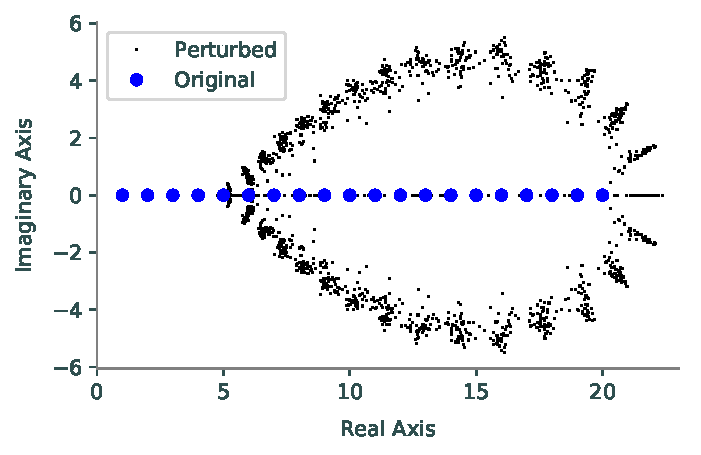
\includegraphics[width=.7\linewidth]{figures/wilkinson_prob_solution.pdf}
\caption{
This figure replicates Figure 12.1 on p. 93 of \cite{Trefethen1997}.}
\label{fig:wilkinsonpolynomial_many}
\end{figure}

\label{prob:wilkinson-polynomial-roots}
\end{problem}

\subsection*{Calculating Eigenvalues} % ---------------------------------------

Let $f:M_n(\mathbb{C}) \rightarrow \mathbb{C}^n$ be the function that maps an $n \times n$ matrix with complex entries to its $n$ eigenvalues.
This problem is well-conditioned for symmetric matrices, but it can be extremely ill-conditioned for non-symmetric matrices.
Let $A$ be an $n\times n$ matrix and let $\boldsymbol{\lambda}$ be the vector of the $n$ eigenvalues of $A$.
If $\tilde{A} = A + H$ is a pertubation of $A$ and $\tilde{\boldsymbol{\lambda}}$ are its eigenvalues, then the condition numbers of $f$ can be estimated by
\begin{equation}
\hat{\kappa}(A) = \frac{\|\boldsymbol{\lambda} - \tilde{\boldsymbol{\lambda}}\|}{\|H\|},
\qquad
\kappa(A) = \frac{\|A\|}{\|\boldsymbol{\lambda}\|}\hat{\kappa}(A).
\label{eq:eig-condition-numbers}
\end{equation}

\begin{problem}\label{prob:eigenvalue} % Eigenvalue experiments
Write a function that accepts a matrix $A$ and estimates the condition number of the eigenvalue problem using (\ref{eq:eig-condition-numbers}).
For the perturbation $H$, construct a matrix with complex entries where the real and imaginary parts are drawn from normal distributions centered at $0$ with standard deviation $\sigma = 10^{-10}$.
\begin{lstlisting}
reals = np.random.normal(0, 1e-10, A.shape)
imags = np.random.normal(0, 1e-10, A.shape)
H = reals + 1j*imags
\end{lstlisting}
Use \li{scipy.linalg.eig()} or \li{scipy.linalg.eigvals()} to compute the eigenvalues of $A$ and $A+H$, and use the 2-norm for both the vector and matrix norms.
Return the absolute and relative condition numbers.
\label{prob:eig-condit}
\end{problem}

\begin{problem}
Write a function that accepts bounds $[x_{\min},x_{\max},y_{\min},y_{\max}]$ and an integer \li{res}.
Use your function from Problem \ref{prob:eig-condit} to compute the relative condition number of the eigenvalue problem for the $2\times 2$ matrix
\[
\left[\begin{array}{cc}
1 &  x\\
y & 1\end{array}\right]
\]
at every point of an evenly spaced \li{res}$\times$\li{res} grid over the domain $[x_{\min}, x_{\max}]\times [y_{\min}, y_{\max}]$.
Plot these estimated relative condition numbers using \li{plt.pcolormesh()} and the colormap \li{cmap='gray_r'}.
With \li{res=200}, your plot should look similar to the following figure.

\begin{figure}[H]
    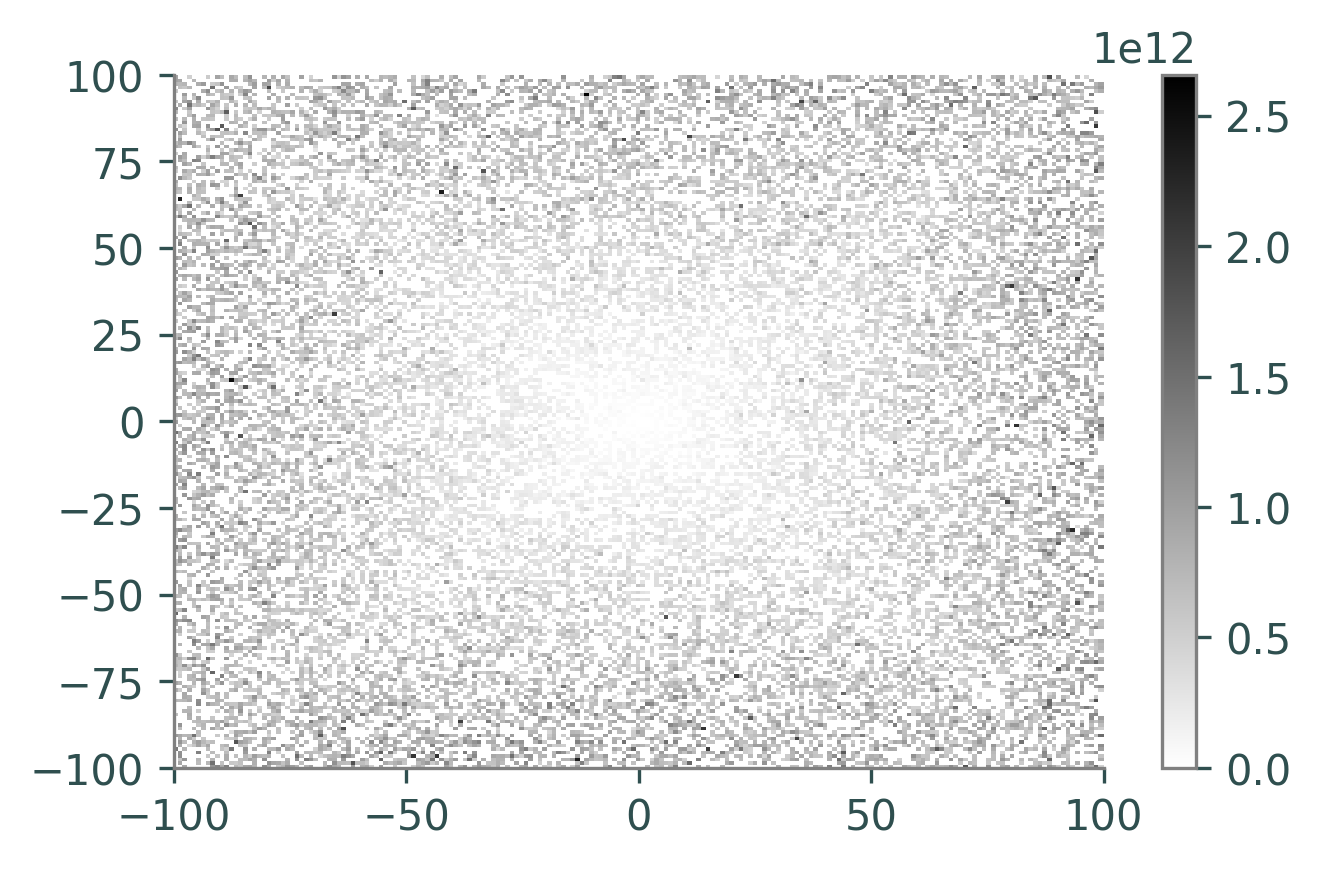
\includegraphics[width=.7\linewidth]{figures/eigenvalue_conditioning.png}
\end{figure}

\label{prob:eigenvalue-conditioning-plot}
\end{problem}

Problem \ref{prob:eigenvalue-conditioning-plot} shows that the conditioning of the eigenvalue problem depends heavily on the matrix, and that it is difficult to know a priori how bad the problem will be.
Luckily, most real-world problems requiring eigenvalues are symmetric.
In their book on Numerical Linear Algebra, L. Trefethen and D. Bau III summed up the issue of conditioning and eigenvalues when they stated, ``\emph{if the answer is highly sensitive to perturbations, you have probably asked the wrong question}.''

\section*{Stability} % ========================================================

The \emph{stability} of an algorithm is measured by the error in its output.
Let $f: \mathbb{R}^m \rightarrow \mathbb{R}^n$ be a problem to be solved, as in the previous section, and let $\tilde{f}$ be an actual algorithm for solving the problem.
The \emph{forward error} of $f$ at $\x$ is $||f(\x)-\tilde f(\x)||$, and the \emph{relative forward error} of $f$ at $\x$ is
\[
\frac{||f(\x)-\tilde f(\x)||}{||f(\x)||}.
\]
An algorithm is called \emph{stable} if its relative forward error is small.%
\footnote{See the Additional Material section for alternative (and more rigorous) definitions of algorithmic stability.}

As an example, consider again NumPy's root-finding algorithm that we used to investigate the Wilkinson polynomial.
The exact roots of $w(x)$ are clearly $1,2,\ldots,20$.
Had we not known this, we could have tried computing the roots from the coefficients using \li{np.roots()} (without perturbing the coefficients at all).

\begin{lstlisting}
# w_coeffs holds the coefficients and w_roots holds the true roots.
>>> computed_roots = np.sort(np.roots(np.poly1d(w_coeffs)))
>>> print(computed_roots[:6])       # The computed roots are close to integers.
[ 1.          2.          3.          3.99999999  5.00000076  5.99998749]

# Compute the forward error.
>>> forward_error = la.norm(w_roots - computed_roots)
>>> print(forward_error)
0.020612653126379665

# Compute the relative forward error.
>>> forward_error / la.norm(w_roots)
0.00038476268486104599              # The error is nice and small.
\end{lstlisting}

This analysis suggests that \li{np.roots()} is a stable algorithm, so large condition numbers of Problem \ref{prob:wilkinson-polynomial-roots} really are due to the poor conditioning of the problem, not the way in which the problem was solved.

\begin{info} % Conditioning versus Stability
Conditioning is a property of a \textbf{problem} to be solved, such as finding the roots of a polynomial or calculating eigenvalues.
Stability is a property of an \textbf{algorithm} to solve a problem, such as \li{np.roots()} or \li{scipy.linalg.eig()}.
If a problem is ill-conditioned, any algorithm used to solve that problem may result in suspicious solutions, even if that algorithm is stable.
\end{info}


\subsection*{Least Squares} % ----------------------------------------
% An example of a problem with stable and unstable algorithms is the least squares problem.

The \emph{ordinary least squares} (OLS) problem is to find the $\x$ that minimizes $\norm{A\x -\b}_2$ for fixed $A$ and $\b$.
It can be shown that an equivalent problem is finding the solution of $A\hrm A\x =A\hrm \b$, called the \emph{normal equations}.
% This is repeated in the problem statement (as it should be).
% \begin{enumerate}
% \item Invert the matrix $A\hrm A$ and then right multiply by $A\hrm \b$ to solve the normal equations.
% Although this approach seems intuitive, it is actually highly unstable and can return an answer with a very large forward error.
%
% \item
% Use the QR-decomposition by factoring the $m\times n$ matrix $A$ of rank $n\geq m$ into $QR$, where $Q$ has orthonormal columns and $R$ is upper triangular.
% It can also be shown that the solution of $R \x = Q\hrm\b$ is equivalent to solving the least squares problem.
% This algorithm has the advantage of being stable.
% \end{enumerate}
A common application of least squares is polynomial approximation.
Given a set of $m$ data points $\{(x_k, y_k)\}_{k=1}^m$, the goal is to find the set of coefficients $\{c_i\}_{i=0}^n$ such that
\[
y_k \approx c_n x_k^n + c_{n-1} x_k^{n-1} + \cdots + c_2 x_k^2 + c_1 x_k + c_0
\]
for all $k$, with the smallest possible error.
These $m$ linear equations yield the linear system
\begin{equation}
A\x =
\left[\begin{array}{cccccc}
x_1^n & x_1^{n-1} & \cdots & x_1^2 & x_1 & 1 \\
x_2^n & x_2^{n-1} & \cdots & x_2^2 & x_2 & 1 \\
x_3^n & x_3^{n-1} & \cdots & x_3^2 & x_3 & 1 \\
\vdots & \vdots & & \vdots & \vdots & \vdots \\
x_m^n & x_m^{n-1} & \cdots & x_m^2 & x_m & 1 \\
\end{array}\right]
\left[\begin{array}{c}
c_n \\ c_{n-1} \\ \vdots \\ c_2 \\ c_1 \\ c_0
\end{array}\right]
=
\left[\begin{array}{c} y_1 \\ y_2 \\ y_3 \\ \vdots \\ y_m \end{array}\right]
= \b.
\label{eq:condstab-poly-leastsq}
\end{equation}

\begin{comment} % Too much detail, they can work this part out.
\begin{lstlisting}
# Use least squares to approximate sin(x) with a five-degree polynomial.
>>> x = np.linspace(0, 6, 10)           # The x-values of the data.
>>> b = np.sin(x) + .2*np.random.randn(10) # The y-values of the data (noisy).
>>> A = np.vander(x, 6)                 # Set up the matrix of data values.
>>> coeffs = la.lstsq(A, b)[0]          # Get the polynomial coefficients.

>>> domain = np.linspace(0, 6, 100)     # Define a finer domain for plotting.
>>> plt.plot(x, b, 'k*')				# Plot the approximated points.
>>> plt.plot(domain, np.sin(domain))

# np.poly1d() converts an array of coefficients into a callable polynomial.
>>> plt.plot(domain, np.poly1d(coeffs)(domain))
\end{lstlisting}
\end{comment}

\begin{problem}
Write a function that accepts an integer $n$.
Solve for the coefficients of the polynomial of degree $n$ that best fits the data found in \texttt{stability\_data.npy}.
Use two approaches to get the least squares solution:

\begin{enumerate}
\item Use \li{la.inv()} to solve the normal equations: $\x = (A\trp A)^{-1}A\trp \b$.
Although this approach seems intuitive, it is actually highly unstable and can return an answer with a very large forward error.

\item Use \li{la.qr()} with \li{mode='economic'} and \li{la.solve_triangular()} to solve the system $R\x = Q\trp\b$, which is equivalent to solving the normal equations.
This algorithm has the advantage of being stable.
\end{enumerate}

Load the data and set up the system (\ref{eq:condstab-poly-leastsq}) with the following code.

\begin{lstlisting}
xk, yk = np.load("stability_data.npy").T
A = np.vander(xk, n+1)
\end{lstlisting}

Plot the resulting polynomials together with the raw data points.
Return the forward error $\norm{A\x-\mathbf{b}}_2$ of both approximations.
\\(Hint: The function \li{np.polyval()} will be helpful for plotting the resulting polynomials.)

Test your function using various values of $n$, taking special note of what happens for values of $n$ near $14$ (pictured below).

\begin{figure}[H]
    \centering
    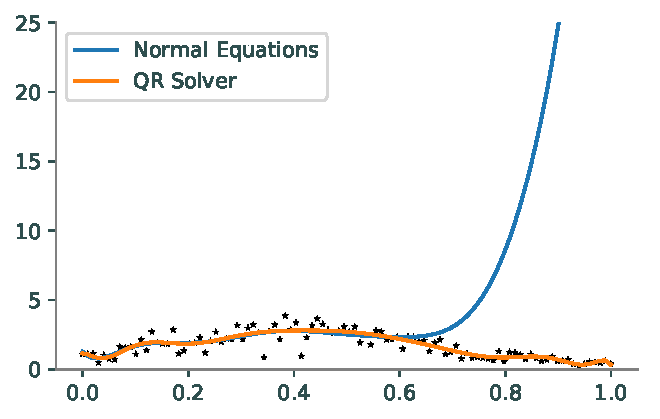
\includegraphics[width=.7\textwidth]{figures/lstsq_stability.pdf}
\end{figure}
\end{problem}

\subsection*{Catastrophic Cancellation} % -------------------------------------

When a computer takes the difference of two very similar numbers, the result is often stored with a small number of significant digits and the tiniest bit of information is lost.
However, these small errors can propagate into large errors later down the line.
This phenomenon is called \emph{catastrophic cancellation}, and is a common cause for numerical instability.

Catastrophic cancellation is a potential problem whenever floats or large integers that are very close to one another are subtracted.
This problem can be avoided by either rewriting the program to not use subtraction, or by increasing the number of significant digits that the computer tracks.

For example, consider the simple problem of computing $\sqrt{a}-\sqrt{b}$.
The computation can be done directly with subtraction, or by performing the equivalent division
\[
\sqrt{a}-\sqrt{b} = (\sqrt{a}-\sqrt{b})\frac{\sqrt{a}+\sqrt{b}}{\sqrt{a}+\sqrt{b}} = \frac{a-b}{\sqrt{a}+\sqrt{b}}.
\]

\begin{lstlisting}
>>> from math import sqrt           # np.sqrt() fails for very large numbers.

>>> a = 10**20 + 1
>>> b = 10**20
>>> sqrt(a) - sqrt(b)               # Do the subtraction directly.
0.0                                 # a != b, so information has been lost.

>>> (a - b) / (sqrt(a) + sqrt(b))   # Use the alternative formulation.
5e-11                               # Much better!
\end{lstlisting}

In this example, $a$ and $b$ are distinct enough that the computer can still tell that $a - b = 1$, but $\sqrt{a}$ and $\sqrt{b}$ are so close to each other that $\sqrt{a} - \sqrt{b}$ is computed as $0$.

\begin{problem}
Let $I(n) = \int_0^1 x^n e^{x - 1} dx$.
It can be shown that for a positive integer $n$,
\begin{equation}
I(n) = (-1)^n(!n - \frac{n!}{e}),
\label{eq:integral-subfactorial-formula}
\end{equation}
where $!n=n!\sum_{k=0}^{n} \frac{(-1)^k}{k!}$ is the \emph{subfactorial} of $n$.
Write a function to do the following.
\begin{enumerate}
\item Use SymPy's \li{sy.integrate()} to evaluate the integral form of $I(n)$ for $n=5,10,\ldots,50$.
Convert the symbolic results of each integration to a float.
Since this is done symbolically, these values can be accepted as the true values of $I(n)$.
\\(Hint: be careful that the values of $n$ in the integrand are of type \li{int}.)

\item Use (\ref{eq:integral-subfactorial-formula}) to compute $I(n)$ for the same values of $n$.
Use \li{sy.subfactorial()} to compute $!n$ and \li{sy.factorial()} to compute $n!$.
\\(Hint: be careful to only pass Python integers to these functions.)
\label{step:subfactorial-cheat}

\item Plot the relative forward error of the results computed in step \ref{step:subfactorial-cheat} at each of the given values of $n$.
Use a log scale on the $y$-axis.
Is (\ref{eq:integral-subfactorial-formula}) a stable way to compute $I(n)$?
Why?
\end{enumerate}
\end{problem}

The examples presented in this lab are just a few of the ways that a mathematical problem can turn into a computational train wreck.
Always use stable algorithms when possible, and remember to check if problems are well conditioned or not.

\begin{comment}
\begin{center}
\begin{tabular}{|l|l|}
\hline
$n$  & Actual value of $I(n)$ \\
\hline
$1$  & $0.367879441171$ \\
$5$  & $0.145532940573$ \\
$10$ & $0.0838770701034$ \\
$15$ & $0.0590175408793$ \\
$20$ & $0.0455448840758$ \\
$25$ & $0.0370862144237$ \\
$30$ & $0.0312796739322$ \\
$35$ & $0.0270462894091$ \\
$40$ & $0.023822728669$ \\
$45$ & $0.0212860390856$ \\
$50$ & $0.0192377544343$ \\
\hline
\end{tabular}
\end{center}

\end{comment}

%\begin{table}
%\centering
%\begin{tabular}{|l|l|l|}
%\hline
%Integrand & Computed Value & Actual Value \\
%\hline
%$x^{1}e^{x}$: & $0.367879441171$ & $0.367879441171$ \\
%$x^{5}e^{x}$: & $0.145532940573$ & $0.145532940573$ \\
%$x^{10}e^{x}$: & $0.0838770701084$ & $0.0838770701034$ \\
%$x^{15}e^{x}$: & $0.0590209960938$ & $0.0590175408793$ \\
%$x^{20}e^{x}$: & $0.0$ & $0.0455448840758$ \\
%$x^{25}e^{x}$: & $1073741824.0$ & $0.0370862144237$ \\
%$x^{30}e^{x}$: & $-1.80143985095 \cdot 10^{16}$ & $0.0312796739322$ \\
%$x^{35}e^{x}$: & $6.04462909807 \cdot 10^{23}$ & $0.0270462894091$ \\
%$x^{40}e^{x}$: & $0.0$ & $0.023822728669$ \\
%$x^{45}e^{x}$: & $0.0$ & $0.0212860390856$ \\
%$x^{50}e^{x}$: & $1.46150163733 \cdot 10^{48}$ & $0.0192377544343$ \\
%\hline
%\end{tabular}
%\caption{Inaccuracy of values computed using an unstable algorithm.}
%\label{table:unstable_computation}
%\end{table}

\newpage

\section*{Additional Material} % ==============================================

\subsection*{Other Notions of Stability} % ------------------------------------

The definition of stability can be made more rigorous in the following way.
Let $f$ be a problem to solve and $\tilde{f}$ an algorithm to solve it.
If for every $\x$ in the domain there exists a $\tilde{\x}$ such that
\[
\frac{\|\tilde{\x} - \x\|}{\|\x\|}
\qquad\text{and}\qquad
\frac{\|\tilde{f}(\x) - f(\tilde{\x})\|}{\|f(\tilde{\x})\|}
\]
are small (close to $\epsilon_{\text{machine}} \approx 10^{-16}$), then $\tilde{f}$ is called stable.
In other words, ``A stable algorithm gives nearly the right answer to nearly the right question'' (Trefethen, Bao, 104).
Note carefully that the quantity on the right is slightly different from the plain forward error introduced earlier.

Stability is desirable, but plain stability isn't the best possible condition.
For example, if for every input $\x$ there exists a $\tilde{\x}$ such that
$\|\tilde{\x} - \x\| / \|\x\|$ is small and $\tilde{f}(\x) = f(\tilde{\x})$ exactly, then $\tilde{f}$ is called \emph{backward stable}.
Thus ``A backward stable algorithm gives exactly the right answer to nearly the right question'' (Trefethen, Bao, 104).
Backward stable algorithms are generally more trustworthy than stable algorithms, but they are also less common.

\begin{comment} % Unfinished garbage table.
\subsection*{Index of Conditioning and Stability of Algorithms} % -------------

\begin{table}[h]
\begin{tabular}{|l|l|l|}
\hline \textbf{Well-Conditioned} & \textbf{Ill-Conditioned} & \textbf{Systems of Equations} \\
{\parbox{0.3\textwidth}{\raggedleft
           \begin{itemize}[leftmargin=*]
               \item finding eigenvalues of a symmetric (or normal) matrix
               \item calculating $e^x$ for relatively small values of $x$
               \item calculating $\ln(x)$ for $x$ not close to $1$
           \end{itemize} }}           &

{\parbox{0.3\textwidth}{\raggedleft
           \begin{itemize}[leftmargin=*]
               \item calculating $x_1 - x_2$ when $x_1 \approx x_2$
               \item computing roots of a polynomial, given the coefficients
               \item computing eigenvalues of a non-symmetric matrix
           \end{itemize} }}              &

{\parbox{0.3\textwidth}{
           \begin{itemize}[leftmargin=*]
                \item relative condition number is \[ \mathcal{K} = ||A|| ||A^{-1}|| \]
           \end{itemize} }}   \\ \hline
\end{tabular}
\end{table}


\begin{table}[h]
\begin{tabular}{|l|l|}
\hline \textbf{Stable} & \textbf{Unstable} \\
{\parbox{0.45\textwidth}{\raggedleft
           \begin{itemize}[leftmargin=*]
               \item finding eigenvalues of a symmetric (or normal) matrix
               \item calculating $e^x$ for relatively small values of $x$
               \item calculating $\ln(x)$ for $x$ not close to $1$
           \end{itemize} }}           &

{\parbox{0.45\textwidth}{\raggedleft
           \begin{itemize}[leftmargin=*]
               \item calculating $x_1 - x_2$ when $x_1 \approx x_2$
               \item computing roots of a polynomial, given the coefficients
               \item computing eigenvalues of a non-symmetric matrix
           \end{itemize} }}    \\ \hline
\end{tabular}
\end{table}
\end{comment}

\subsection*{Stabilty of Linear System Solvers} % -----------------------------

The algorithms presented so far in this manual have different levels of stability.
The LU decomposition (with pivoting) is usually very good, but there are some pathological examples of matrices that can cause it to break down.
Even so, \li{scipy.linalg.solve()} uses the LU decomposition.
The QR decomposition (also with pivoting) is generally considered to be a better option than the LU decomposition and is more stable.
However, solving a linear system using the SVD is even more stable than using the QR decomposition.
For this reason, \li{scipy.linalg.lstsq()} uses the SVD.
